\newcommand{\dtBar}{\overline{\dt}}
\section{Performance Results}\label{sec:performanceResults}

The normalized measure of CPU,  {\em time-to-solution} (TTS), defined below,
can be used to compare results from different time-stepping schemes, different numbers of processors and even different grids. 
Smaller values of TTS correspond to faster schemes. 
\begin{eqnarray*}
 \Nc_g &=& \mbox{number of grid points}, \\
  N_p &=& \mbox{number of processors}, \\
  N_s &=& \mbox{number of time steps}, \\
  \dtBar  &=& t_{\rm final}/N_s =  \mbox{average time-step}, \\
  \dt_a  &=& \mbox{velocity-scale}/\mbox{average grid spacing} = \mbox{time-step scale for advection}, \\
 \mbox{TPS} &=& \mbox{total-wall-clock-time}/N_s = \mbox{average CPU time (s) per step}, \\
 \mbox{TPSM} &=& \mbox{average CPU time (s) per step per million grid points per processor}, \\
              &=& N_p \times \mbox{TPS}/( \Nc_g/10^6) , \\
 \mbox{TTS} &=&  \mbox{normalized average CPU time (s) to solve}, \\
            &=& \mbox{TPSM} \times \dt_a/\dtBar
\end{eqnarray*}


The {\em normalized memory usage},  RPG, measures the number of {\em reals-per-grid-point} (i.e. the equivalent 
number of double precision values (8 bytes, 64 bits) per grid point) for the entire memory use. 
\begin{eqnarray*}
 \mbox{RPG} &=& (\mbox{total memory usage (btyes)})/(\mbox{number-of-grid-points} \times (8~\mbox{bytes/real}))
\end{eqnarray*}

\subsection{Performance: two cylinders in a channel} \label{sec:performanceTwoCylinders}

% --- SEE runs/cgins/compare/memo.tcilc16
\begin{table}[hbt]
\begin{center}
\begin{tabular}{|c|c|c|c|c|c|c|c|} \hline 
   Grid          &  Pts     & Method   & P-solver  &   $N_p$  & TPSM     & TTS      &  RPG      \\ \hline
 tcilce16        & $1.4$M   & IM22     &  BICGS(3) &  serial  & $18 $    & $54 $    & $200$     \\ 
                 &          & PC22     &  BICGS(3) &  serial  & $9.6$    & $62 $    & $67 $     \\ 
                 &          & IM24     &  BICGS(3) &  serial  & $32 $    & $170$    & $314$     \\ 
                 &          & IM24     &  MG       &  serial  & $5.5$    & $29 $    & $171$     \\ 
                 &          & IM24MG   &  MG       &  serial  & $3.9$    & $20 $    & $49 $     \\ 
                 &          & AFS22    &  MG       &  serial  & $11 $    & $16 $    & $27 $     \\ 
                 &          & AFS24    &  MG       &  serial  & $13 $    & $21 $    & $31 $     \\ 
\hline 
\end{tabular}
\end{center}
\caption{Performance of Cgins for different time-stepping methods and different linear solvers for the
   pressure equation. TTS is the normalized time-to-solution. 
RPG is the total memory usage in reals-per-grid-point.
}
\label{tab:performanceTcilc16} 
\end{table}

% \begin{table}[hbt]
% \begin{center}
% \begin{tabular}{|c|c|c||c|c|c||c|c|c|c|} \hline 
% %     & & & \multicolumn{2}{|c|}{CPU: TR10M} &   & \multicolumn{2}{|c|}{Mem: RPG} &   Memory  \\
%                  &          &          & Pressure  &  IM22    & IM22   &   AFS22  & AFS22   &  AFS42 & AFS42  \\ 
%    Grid          &  Pts     &  $N_p$   &  Solver   &  TTS     & RPG    &   TTS    &  RPG    &  TTS   &  RPG   \\ \hline
%  tcilce16        & $1.4$M   & serial   &  BICGS(3) & $7.2$    & $107$  & $7.3$    & $ 63 $  & $8.6$  &        \\ 
% \hline 
% \end{tabular}
% \end{center}
% \caption{Performance of Cgins for solving various problems.
% RPG is the total memory usage in reals-per-grid-point.
% }
% \label{tab:performanceSecondOrder} 
% \end{table}

\begin{figure}[hbt]
\begin{center}
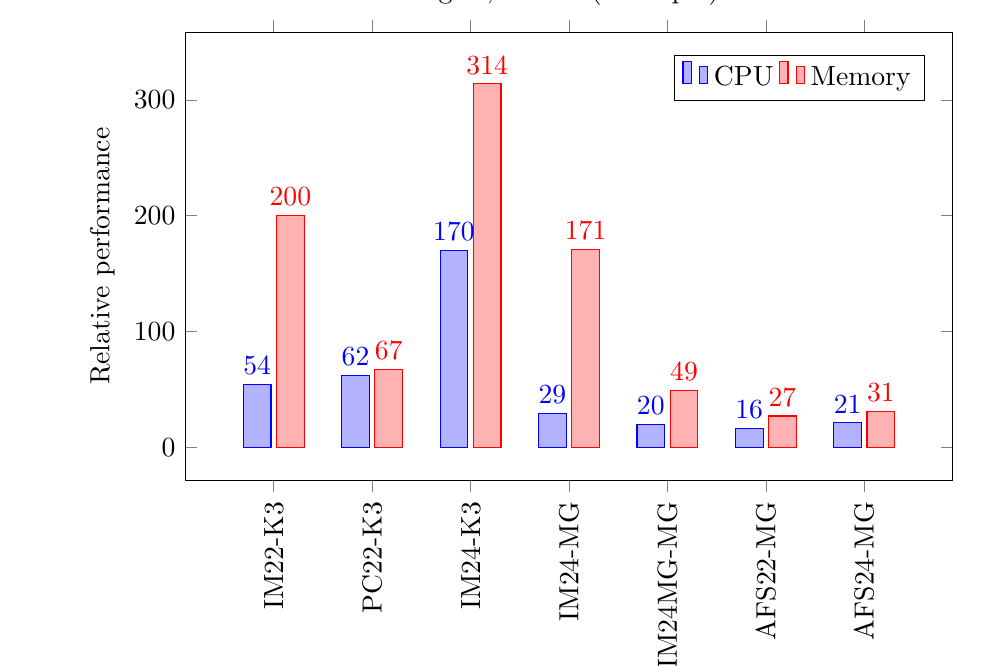
\begin{tikzpicture}
\useasboundingbox (-2,-2.0) rectangle (10,5.75);  % set the bounding box (so we have less surrounding white space)
\begin{axis}[
      ybar,
      x=1.25cm, % distance between entries?
      enlargelimits=0.15,
      legend style={at={(0.80,0.95)}, % location of legend
          anchor=north,legend columns=-1},
      ylabel={Relative performance},
      symbolic x coords={IM22-K3,PC22-K3,IM24-K3,IM24-MG,IM24MG-MG,AFS22-MG,AFS24-MG},
      xtick=data,
      x tick label style= {rotate=90,anchor=east},  % rotate bottom ``tick'' labels
      nodes near coords,
      nodes near coords align={vertical},
      title={Cgins, tcilc16 (1.4M pts)}
      ]
\addplot coordinates { (IM22-K3, 54) (PC22-K3, 62) (IM24-K3,170) (IM24-MG, 29) (IM24MG-MG, 20) (AFS22-MG, 16) (AFS24-MG, 21) };
\addplot coordinates { (IM22-K3,200) (PC22-K3, 67) (IM24-K3,314) (IM24-MG,171) (IM24MG-MG, 49) (AFS22-MG, 27) (AFS24-MG, 31) };
% \addplot coordinates {(tool8,4) (tool9,4) (tool10,4)};
% \addplot coordinates {(tool8,1) (tool9,1) (tool10,1)};
\legend{CPU,Memory}
\end{axis}
% \draw (current bounding box.south west) rectangle (current bounding box.north east);
% \draw[step=1cm,gray] (-2,-2) grid (7,6);
\end{tikzpicture}
\end{center}
\caption{Performance of Cgins for different time stepping methods for flow past two cylinders in a channel.
   The CPU is a normalized time-to-solution (TTS). 
   The memory usage is measured in reals-per-grid-point. K3 stands for the Krylov solver BiCGStab-ILU(3). 
}
\label{fig:performanceTcilc16} 
\end{figure}


% --- SEE runs/cgins/compare/memo.tcilc646
\begin{table}[hbt]
\begin{center}
\begin{tabular}{|c|c|c|c|c|c|c|c|} \hline 
   Grid          &  Pts     & Method   & P-solver  &   $N_p$  & TPSM     & TTS      &  RPG      \\ \hline
 tcilce64        & $22.$M   & PC24     &  BICGS(5) &  $16$    & $840$    & $16000$  & $205$     \\ 
                 &          & PC24     &  MG       &  $16$    & $15$     & $210$    & $67 $     \\ 
%                &          & IM24     &  BICGS(3) &  serial  &          & $170$    & $314$     \\ 
%                &          & IM24     &  MG       &  serial  &          & $29 $    & $171$     \\ 
                 &          & IM24MG   &  MG       &  $16$    & $34$     & $180$    & $46 $     \\ 
%                &          & AFS22    &  MG       &  serial  &          & $16 $    & $27 $     \\ 
                 &          & AFS24    &  MG       &  $16$    & $34$     & $54 $    & $32 $     \\ 
\hline 
\end{tabular}
\end{center}
\caption{Performance of Cgins for different time-stepping methods and different linear solvers for the
   pressure equation. TTS is the normalized time-to-solution. 
RPG is the total memory usage in reals-per-grid-point.
}
\label{tab:performanceVariousProblems} 
\end{table}
Table~\ref{tab:performanceVariousProblems} gives performance results for grid {\tt tcilce64.order4.ml4}. 
NOTE: Case IM24MG-MG was run at $\nu=10^{-4}$ while the other cases were run at $\nu=10^{-5}$ so the
value of TTS is not exactly comparable.


% -------------------------------------------------------------------------------------------------------
\newcommand{\Gcj}{\Gc_j}
\subsection{Performance: pitching-plunging airfoil} \label{sec:performancePitchingPlungingAirfoil}


We consider flow past a two-dimensional Joukowsky airfoil that undergoes a pitching and
plunging motion. Let $\Gcj^{(j)}$ denote the grid for this problem with target grid
spacing of $\ds=.05/j$. 

Grid $\Gcj^{(16)}$ has approximately $1.7$M grid points.
Grid $\Gcj^{(32)}$ has approximately $6.8$M grid points.

% --- SEE runs/cgins/compare/memo.wing
\begin{table}[hbt]
\begin{center}
\begin{tabular}{|c|c|c|c|c|c|c|c|} \hline 
   Grid          &  Pts     & Method   & P-solver  &   $N_p$  & TPSM     & TTS      &  RPG      \\ \hline
 joukowsky16     & $1.7$M   & AFS24    &  BICGS(5) &  $8 $    & $340$    & $1,700$ & $246$     \\ 
                 &          & AFS24    &  MG       &  $8 $    & $29 $    & $140$  & $79 $     \\ 
\hline
 joukowsky32     & $6.8$M   & AFS24    &  BICGS(5) &  $16$    & $660$    & $3,700$ & $235$     \\ 
                 &          & AFS24    &  MG       &  $16$    & $ 40$    & $230 $ & $ 65$     \\ 
                 &          & AFS24    &  MG       &  $ 8$    & $ 32$    & $  99 $ & $ 54$     \\ 
\hline 
\end{tabular}
\end{center}
\caption{Performance of Cgins for different time-stepping methods and different linear solvers for the
   pressure equation. TTS is the normalized time-to-solution. 
RPG is the total memory usage in reals-per-grid-point.
}
\label{tab:performancePitchingPlunging} 
\end{table}


% --- SEE runs/cgins/compare/memo.wing
\begin{table}[hbt]
\begin{center}
\begin{tabular}{|c|c|c|c|c|c|c|c|} \hline 
   Grid          &  Pts     & Method   & P-solver  &   $N_p$  & TPSM     & TTS      &  RPG      \\ \hline
 joukowsky32     & $6.8$M   & AFS24    &  BICGS(5) &  $16$    & $1100$   & $1800$   & $235$     \\ 
                 &          & AFS24    &  MG       &  $16$    & $ 52$    & $ 76 $   & $ 66$     \\ 
\hline 
\end{tabular}
\end{center}
\caption{RESTART. Performance of Cgins for different time-stepping methods and different linear solvers for the
   pressure equation. TTS is the normalized time-to-solution. 
RPG is the total memory usage in reals-per-grid-point.
}
\label{tab:performancePitchingPlungingII} 
\end{table}